\documentclass{beamer}

\mode<presentation> {
  \usetheme{Madrid}
}

\usepackage{graphicx} % Allows including images
\usepackage{booktabs} % Allows the use of \toprule, \midrule and \bottomrule in tables
\usepackage{amsmath,amssymb}
\usepackage{etoolbox}
\usepackage{algorithm}
\usepackage{algorithmic}
\usepackage{tikz}
\usepackage{xcolor}

\usetikzlibrary{arrows,fadings,shadings,positioning,calc,decorations.pathmorphing}

\newcommand\Pitem{%
  \addtocounter{enumi}{-1}%
  \renewcommand\theenumi{\arabic{enumi}'}%
  \item%
  \renewcommand\theenumi{\arabic{enumi}}%
}

\renewcommand\algorithmicrequire{\textbf{Input: }}

\usepackage{mathutils}

\usepackage[style=british]{csquotes}

\def\signed #1{{\leavevmode\unskip\nobreak\hfil\penalty50\hskip1em
  \hbox{}\nobreak\hfill #1%
  \parfillskip=0pt \finalhyphendemerits=0 \endgraf}}

\newsavebox\mybox
\newenvironment{aquote}[1]
  {\savebox\mybox{#1}\begin{quote}\openautoquote\hspace*{-.7ex}}
  {\unskip\closeautoquote\vspace*{1mm}\signed{\usebox\mybox}\end{quote}}

\def\Actions{\mathcal{A}}
\def\BH{\widehat{B}}
\def\KH{\widehat{\mathcal{K}}}
\def\Xop{\mathfrak{X}}
\def\Bbar{\bar{B}}
\def\Bhat{\BH}
\def\Hist{\mathcal{H}}
\def\Xmat{\mathbf{X}}

\def\II{\mathbb{I}}

\def\Aset{\mathcal{A}}
\def\Bset{\mathcal{B}}
\def\Cset{\mathcal{C}}
\def\Dset{\mathcal{D}}
\def\Eset{\mathcal{E}}
\def\Fset{\mathcal{F}}
\def\Gset{\mathcal{G}}
\def\Hset{\mathcal{H}}
\def\Kset{\mathcal{K}}
\def\Oset{\mathcal{O}}
\def\Sset{\mathcal{S}}

\def\gmax{\gamma_{\max{}}}
\def\gmin{\gamma_{\min{}}}

\def\gtmax{\tilde{\gamma}_{\max{}}}
\def\gtmin{\tilde{\gamma}_{\min{}}}

\def\Dball{\mathfrak{D}}

\def\Bhat{\widehat{B}}
\def\Xtilde{\widetilde{X}}
\def\Bbar{\bar{B}}
\def\P{\mathcal P}

\def\d{d}
\def\k{k}
\def\l{l}
\def\p{p}

\def\Orth{{\sf O}}
\def\Cone{\mathcal{C}}
\def\Constraint{\mathfrak{C}}
\def\spike{\alpha_{\operatorname{sp}}}
\def\ratio{\beta_{\operatorname{ra}}}
\def\xmax{x_{\max{}}}
\def\xtmax{\widetilde{x}_{\max{}}}
\def\epsmax{\eps_{\max{}}}
\def\rowmatrix{row-matrix}

\def\B{B}
\def\Loss{\mathcal{L}}

\newcommand\independent{\protect\mathpalette{\protect\independenT}{\perp}}
\def\independenT#1#2{\mathrel{\rlap{$#1#2$}\mkern2mu{#1#2}}}

\def\eps{\varepsilon}

\newtheorem{assumes}[theorem]{Assumption}


\title[REAL-Bandit]{Many-Armed Bandits with High-Dimensional Contexts under a Low-Rank Structure}

\author[N. Hamidi, M. Bayati, K. Gupta]{Nima Hamidi\\{\scriptsize Stanford University}\\\vskip3mm
Mohsen Bayati\\{\scriptsize Stanford University}\\\vskip3mm
Kapil Gupta\\{\scriptsize Airbnb}}
\date{}

\begin{document}


\begin{frame}
\titlepage % Print the title page as the first slide
\end{frame}

\begin{frame}{Formal setting}
\begin{enumerate}
    \item Each arm $i$ corresponds to an \textbf{unknown} vector $B_i\in\IR^d$.
    \vskip7mm
    \item At time $t$, a \textbf{context vector} $X_t\in\IR^d$ is revealed to the policy.
    \vskip7mm
    \item The policy $\pi$ selects action $a_t\in[k]$.
    \vskip7mm
    \item The \textbf{reward} is given by $y_t=\inner{B_{a_t}, X_t}+\varepsilon_{t}$.
\end{enumerate}
\pause
\bigskip

We further assume:
\begin{enumerate}
\item $X_t$'s are i.i.d.
\item $\varepsilon_t$'s are independent mean-zero sub-Gaussian.
\item $(X_t)\independent(\varepsilon_t)$
\item $B$ is of rank $r$.
\end{enumerate}

\end{frame}

\begin{frame}{Cumulative regret}
\begin{definition}
We define the \textbf{cumulative regret} of a given policy as follows:
\begin{align*}
R_T=\sum_{t=1}^T\left[\max_{1\leq i\leq k}\inner{B_{t,i},X_t}-\inner{B_{t,a_t},X_t}\right].
\end{align*}
\end{definition}
Policies with smaller (expected) regrets are desired.
\end{frame}

\begin{frame}{Theoretical guarantees}
    \begin{itemize}
        \item OLS-Bandit: $O(d^2k^3\log(T))$ {\color{blue}\cite{ols-bandit}}
        \vskip7mm
        \item Lasso-Bandit: $O(s^2k^3\log(T)^2)$ {\color{blue}\cite{lasso-bandit}}
        \vskip7mm
        \item REAL-Bandit: $O(r^2(k+d)\log(T)^2)$
    \end{itemize}
\end{frame}

\section{REAL-Bandit and Theoretical Results}
\begin{frame}{REAL-Bandit}
\begin{figure}[H]
\centering
\begin{tikzpicture}
  [
  default/.style={fill=black!20!white,draw=white!50!black,minimum width=5mm,anchor=west},
  forced/.style={fill=green!20!white,draw=green!50!black,minimum width=5mm,anchor=west},
   all/.style={fill=blue!20!white,draw=blue!50!black,minimum width=5mm,anchor=west},
   arm/.style={fill=red!20!white,draw=red,anchor=north,circle,minimum width=3mm,inner sep=0.5mm,yshift=-1mm}]
\onslide<+->{
    \node [default](m1) {\scriptsize 1};
    \node [default](m2) at (m1.east) {\scriptsize 2};
    \node [default](m3) at (m2.east) {\scriptsize 3};
    \node [default](m4) at (m3.east) {\scriptsize 4};
    \node [default](m5) at (m4.east) {\scriptsize 5};
    \node [default](m6) at (m5.east) {\scriptsize 6};
    \node [default](m7) at (m6.east) {\scriptsize 7};
    \node [default](m8) at (m7.east) {\scriptsize 8};
    \node [default](m9) at (m8.east) {\scriptsize 9};
    \node [default](m10) at (m9.east) {\scriptsize 10};
    \node [default](m11) at (m10.east) {\scriptsize 11};
    \node [default](m12) at (m11.east) {\scriptsize 12};
    \node [default](m13) at (m12.east) {\scriptsize 13};
    \node [default](m14) at (m13.east) {\scriptsize 14};
    \node [default](m15) at (m14.east) {\scriptsize 15};
    \node [default](m16) at (m15.east) {\scriptsize 16};
    \node [default](m17) at (m16.east) {\scriptsize 17};
    \node [default](m18) at (m17.east) {\scriptsize 18};
    \node [default](m19) at (m18.east) {\scriptsize 19};
    \node [default](m20) at (m19.east) {\scriptsize 20};
}
\onslide<+->{
    \node [forced](n1) {\scriptsize 1};
    \node [forced](n2) at (n1.east) {\scriptsize 2};
    \node [forced](n3) at (n2.east) {\scriptsize 3};
    \node [forced](n4) at (n3.east) {\scriptsize 4};
    \node [all](n5) at (n4.east) {\scriptsize 5};
    \node [forced](n6) at (n5.east) {\scriptsize 6};
    \node [all](n7) at (n6.east) {\scriptsize 7};
    \node [all](n8) at (n7.east) {\scriptsize 8};
    \node [all](n9) at (n8.east) {\scriptsize 9};
    \node [all](n10) at (n9.east) {\scriptsize 10};
    \node [all](n11) at (n10.east) {\scriptsize 11};
    \node [all](n12) at (n11.east) {\scriptsize 12};
    \node [forced](n13) at (n12.east) {\scriptsize 13};
    \node [all](n14) at (n13.east) {\scriptsize 14};
    \node [all](n15) at (n14.east) {\scriptsize 15};
    \node [all](n16) at (n15.east) {\scriptsize 16};
    \node [all](n17) at (n16.east) {\scriptsize 17};
    \node [all](n18) at (n17.east) {\scriptsize 18};
    \node [forced](n19) at (n18.east) {\scriptsize 19};
    \node [all](n20) at (n19.east) {\scriptsize 20};
}
\onslide<+->{
    \node [arm] at (n1.south) {\scriptsize 1};
    \node [arm] at (n2.south) {\scriptsize 2};
    \node [arm] at (n3.south) {\scriptsize 3};
    \node [arm] at (n4.south) {\scriptsize 1};
    \node [arm] at (n5.south) {\scriptsize 1};
    \node [arm] at (n6.south) {\scriptsize 3};
    \node [arm] at (n7.south) {\scriptsize 1};
    \node [arm] at (n8.south) {\scriptsize 2};
    \node [arm] at (n9.south) {\scriptsize 3};
    \node [arm] at (n10.south) {\scriptsize 1};
    \node [arm] at (n11.south) {\scriptsize 2};
    \node [arm] at (n12.south) {\scriptsize 3};
    \node [arm] at (n13.south) {\scriptsize 2};
    \node [arm] at (n14.south) {\scriptsize 3};
    \node [arm] at (n15.south) {\scriptsize 1};
    \node [arm] at (n16.south) {\scriptsize 2};
    \node [arm] at (n17.south) {\scriptsize 2};
    \node [arm] at (n18.south) {\scriptsize 2};
    \node [arm] at (n19.south) {\scriptsize 3};
    \node [arm] at (n20.south) {\scriptsize ?};
}
\end{tikzpicture}
\end{figure}
\begin{figure}[H]
\centering
\begin{tikzpicture}
  [arm/.style={fill=red!20!white,draw=red,circle,yshift=-6mm},
   histf/.style={fill=green!20!white,draw=green!50!black,yshift=4mm,xshift=-5mm},
   hista/.style={fill=blue!20!white,draw=blue!50!black,yshift=-4mm,xshift=-5mm},
   estf/.style={xshift=2.2cm,anchor=west,yshift=4mm},
   esta/.style={xshift=3.2cm,anchor=west,yshift=-4mm},
   filter/.style={fill=green!20!white,draw=green!50!black,xshift=1.3cm},
   argmax/.style={fill=blue!20!white,draw=blue!50!black},
   linef/.style={dashed,green!40!black},
   linea/.style={dashed,blue!20!black}]
\onslide<4-9>{
    \node [arm] (arm1) {1};
    \node [arm, below of=arm1] (arm2) {2};
    \node [arm, below of=arm2] (arm3) {3};
    
    \node [histf,right=of arm1] (histf1) {1, 4};
    \node [hista,right=of arm1] (hista1) {5, 7, 10, 15};
    \node [histf,right=of arm2] (histf2) {2, 13};
    \node [hista,right=of arm2] (hista2) {8, 11, 16, 17, 18};
    \node [histf,right=of arm3] (histf3) {3, 6, 19};
    \node [hista,right=of arm3] (hista3) {9, 12, 14};
    
    \draw (arm1.east) -- ++(3mm,0) -- ++(0,4mm) -- (histf1.west);
    \draw (arm1.east) -- ++(3mm,0) -- ++(0,-4mm) -- (hista1.west);
    \draw (arm2.east) -- ++(3mm,0) -- ++(0,4mm) -- (histf2.west);
    \draw (arm2.east) -- ++(3mm,0) -- ++(0,-4mm) -- (hista2.west);
    \draw (arm3.east) -- ++(3mm,0) -- ++(0,4mm) -- (histf3.west);
    \draw (arm3.east) -- ++(3mm,0) -- ++(0,-4mm) -- (hista3.west);
}

\onslide<5,8>{
    \node [estf,right=of arm1] (estf1) {\color{green!40!black}$\BH^F_{20,1}$};
    \node [estf,right=of arm2] (estf2) {\color{green!40!black}$\BH^F_{20,2}$};
    \node [estf,right=of arm3] (estf3) {\color{green!40!black}$\BH^F_{20,3}$};
    
    \draw [linef,->] (histf1.east) -- (estf1.west);
    \draw [linef,->] (histf2.east) -- (estf2.west);
    \draw [linef,->] (histf3.east) -- (estf3.west);
}

\onslide<6,9>{
    \node [esta,right=of arm1] (esta1) {\color{blue!20!black}$\BH^A_{20,1}$};
    \node [esta,right=of arm2] (esta2) {\color{blue!20!black}$\BH^A_{20,2}$};
    \node [esta,right=of arm3] (esta3) {\color{blue!20!black}$\BH^A_{20,3}$};
    
    \draw [linea,->] (hista1.east) -- (esta1.west);
    \draw [linea,->] (hista2.east) -- (esta2.west);
    \draw [linea,->] (hista3.east) -- (esta3.west);
}

\onslide<7-9>{
    \node [filter,right=of estf2] (filter) {filter};
    \node [argmax,below=of filter] (argmax) {argmax};
}

\onslide<8>{
    \draw [linef] (estf1.east) -- (filter.west);
    \draw [linef] (estf2.east) -- (filter.west);
    \draw [linef] (estf3.east) -- (filter.west);
}

\onslide<9>{
	\draw [linea] (esta1.east) -- (argmax.west);
	\draw [linea] (esta3.east) -- (argmax.west);
}

\onslide<7-9>{
    \draw [->, thick] (filter.south) -- (argmax.north) node [right,midway] {$\scriptscriptstyle\KH=\{ \inner[small]{\BH^F_{t,\kappa},X_t}\geq\max_{\kappa'}\inner[small]{\BH^F_{t,\kappa'},X_t}-h \}$};
    \draw [->] (argmax.east) -- ++(4mm, 0) node [right] {$a_{20}$};
}
\end{tikzpicture}
\end{figure}
\end{frame}

\begin{frame}{REAL-Estimator}
\begin{itemize}
    \item Use any low-rank estimator, such as
    \begin{align*}
    \bar{B}:=\argmin_{B}\frac{\norm[small]{Y-\Xop(B)}_2^2}{n}+\lambda\normNuc{B}
    \end{align*}
    such that the following holds with high probability
    \begin{align*}
        \normF{\bar{B}-B}^2\leq C\sigma^2\frac{dr}{n}.
    \end{align*}
    \item This bound leads to extra $\sqrt k$ in the regret bound.
\end{itemize}
\end{frame}

\begin{frame}{REAL-Estimator}
\begin{itemize}
    \item Let $\bar{B}$ be defined as in the previous slide.
    \vskip5mm
    \item Run the following ``\emph{row-enhancement}'' procedure.
    \vskip5mm
    \item This procedure eliminates extra $\sqrt k$ factor in the regret.
\end{itemize}
\begin{figure}
    \begin{algorithmic}[1]
    \REQUIRE matrix $\Bbar_{k\times d}$, observations $(X_1,Y_1),\cdots,(X_{n},Y_{n})$
    \STATE Compute SVD $\Bbar=UDV^T$.
    \STATE Let $V_r^T$ be the matrix containing $r$ top rows of $V^T$.
    \STATE Let $\hat\beta=\argmin_{\beta\in\IR^d}\sum_{i=1}^{n}(Y_i-X_iV_r\beta)^2$.
    \STATE Then, output $\Bhat_\kappa=(V_r\hat\beta)^T$.
    \end{algorithmic}
\end{figure}
\end{frame}

\begin{frame}{REAL-Estimator}
\begin{figure}[h]
\centering
\begin{tikzpicture}[
    node distance=-\pgflinewidth,
    data/.style={
        draw=red,
        fill=red!20!white,
        minimum height=3cm,
        inner sep=3pt
    },
    bigmat/.style={fill=blue!20!white,draw=blue,
                   minimum height=2.5cm,
                   minimum width=2.5cm,
                   inner sep=3pt},
    tallmat/.style={fill=gray!50!white,draw=gray,
                    minimum height=2.5cm,
                    minimum width=0.5cm,
                    inner sep=3pt},
    smallmat/.style={fill=gray!50!white,draw=gray,
                     minimum height=0.5cm,
                     minimum width=0.5cm,
                     inner sep=3pt},
    widemat/.style={fill=gray!50!white,draw=gray,
                    minimum height=0.5cm,
                    minimum width=2.5cm,
                    inner sep=3pt},
    awidemat/.style={fill=green,draw=green!50!black,
                     minimum height=0.5cm,
                     minimum width=2.5cm,
                     inner sep=3pt},
    atallmat/.style={fill=green,draw=green!50!black,
                     minimum height=2.5cm,
                     minimum width=0.5cm,
                     inner sep=3pt},
]
\onslide<+->{
    \node [data] (data1) {Data 1};
    \node [data, below=of data1] (data2) {Data 2};
}

\onslide<+->{
    \node [bigmat, right=of data1,xshift=2cm] (bbar) {$\bar{B}$};
     \draw [->,decorate,
    decoration={snake,amplitude=.4mm,segment length=2mm,post length=1mm}] ($(data1.east)+(2mm,0mm)$) -- ($(bbar.west)-(2mm,0mm)$);
}


\onslide<+->{
    \node [right=of bbar,xshift=2mm] (eq) {$=$};
    \node [tallmat, right=of eq,xshift=2mm] (umat) {$U$};
    \node [smallmat, right=of umat,xshift=2mm,yshift=1cm] (dmat) {$D$};
    \node [widemat, right=of dmat,xshift=2mm] (vmat) {$V$};
}

\onslide<+->{
    \node [awidemat, right=of dmat,xshift=2mm] (avmat) {$V$};
}

\onslide<+->{
    \node [awidemat, below=of avmat,yshift=-2.5cm] (alvmat) {$V$};
     \draw [->,decorate,
    decoration={snake,amplitude=.4mm,segment length=2mm,post length=1mm}] ($(avmat.south)-(0mm,2mm)$) -- ($(alvmat.north)+(0mm,2mm)$);
}

\onslide<+->{
    \node [atallmat, below=of umat,yshift=-5mm] (smat) {$S$};
    \node [left=of smat,xshift=-2mm] (aeq) {$=$};
    \node [bigmat, below=of bbar,yshift=-5mm] (bhat) {$\widehat{B}$};
     \draw [->,decorate,
    decoration={snake,amplitude=.4mm,segment length=2mm,post length=1mm}] ($(data2.east)+(2mm,0mm)$) -- ($(bhat.west)-(2mm,0mm)$);
}
\end{tikzpicture}
\end{figure}\end{frame}


\section{Simulations}

\begin{frame}{Simulations}
\begin{itemize}
\item $B$: $200\times 201$ of rank $3$,
\item SD of noise ($\sigma$): 1,
\item Context vectors ($X_t$): vectors of length 201 with i.i.d. standard normal entries.
\end{itemize}
\begin{figure}[H]
  \centering
  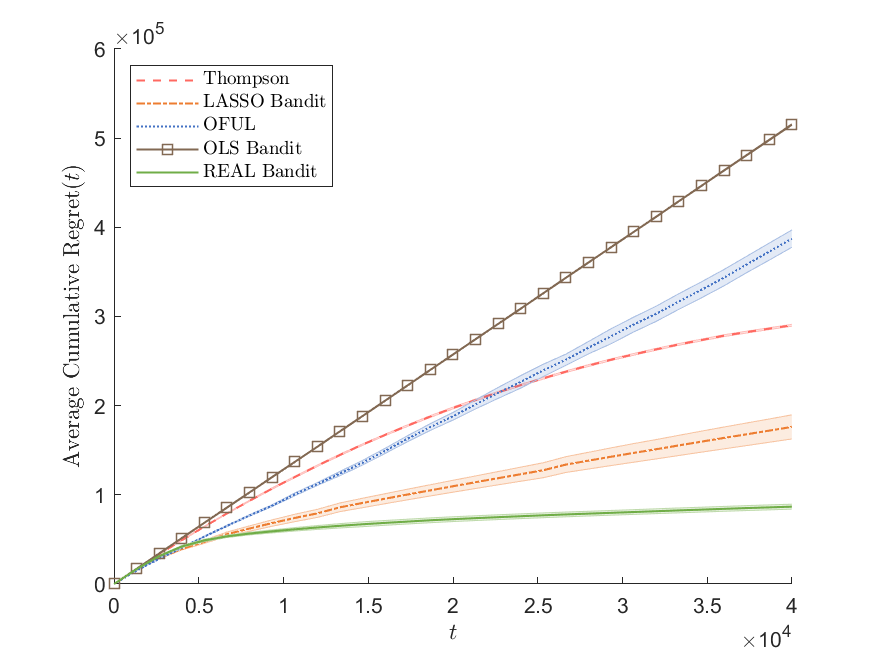
\includegraphics[scale=0.5]{images/regrets.png}
\end{figure}
\end{frame}

\begin{frame}
\frametitle{References}
\footnotesize{
\begin{thebibliography}{99}
\bibitem[Alexander Goldenshluger]{ols-bandit} Alexander Goldenshluger and Assaf Zeevi
\newblock \emph{A linear response bandit problem}
\newblock Stochastic Systems 3.1 (2013): 230-261.
%
\bibitem[Hamsa Bastani]{lasso-bandit} Hamsa Bastani and Mohsen Bayati
\newblock \emph{Online decision-making with high-dimensional covariates}
\newblock (2015).
\end{thebibliography}
}
\end{frame}

\begin{frame}
\Huge{\centerline{Thank you}}
\end{frame}

\end{document}